In this chapter, theory related to multicore architecture and parallel programming is
explained in order to give the reader the foundation needed to understand these aspects of
the thesis.

\section{Multicore architecture}
\subsection{Processes vs threads}
While both threads and processes represent contexts in which a program is run, they have a few differences. A thread is run inside
a process, and the threads within the process share memory and state with each other and the parent
process \cite{singh_2013_parallel_padpwprfmm}. Individual processes do not share memory with each other, and any
communication between processes must be done with message passing rather than with shared memory. Consequently, communication
between threads is generally faster than between processes.
Typically, different threads can be scheduled on different cores, which is also true for different processes.

\subsection{Multicore communication and caching}
Multiple processors communicate with each other through a bus or a network \cite[p. 472-476]{herlihy_2012_art_taomprr}. Since the
means of communication between the processes is a finite resource, too much traffic may result in delays. The processors typically
have their own cache. In order to avoid unnecessary reads from the slower main memory, processors may read from another processor
that has the requested data cached. In a process called \emph{cache coherence}, shared cached values are kept up to date using one
of several protocols. The effect that these different means of communication between processors has on performance in
multiprocessor programs should not be ignored.

\section{Parallel shared memory programming}

\subsection{Data parallelism}
Data parallelism denotes code where the parallelism comes from decomposing the data and running it with the same piece of code
across several processors or computers \cite{singh_2013_parallel_padpwprfmm}. It allows scalability as number of cores and problem
sizes increase, since more parallelism can be exploited for larger datasets \cite[p. 24]{mccool_2012_structured_spppfec}.

\subsection{Task parallelism}
In task parallelism, groups of tasks that are independent are run in parallel \cite{chow_2015_pipeline_ppiaote}.
Tasks that depend on each other cannot be run in parallel, and must instead be run sequentially.
A group of tasks is embarrassingly parallel if none of the tasks in the group depend on each other.

\subsection{Scheduling}
Threads and processes are scheduled by the operating system, and the exact mechanism for choosing what to schedule when differs
between platforms and implementations \cite[p. 472]{herlihy_2012_art_taomprr}. Scheduling may imply running truly parallel
on different cores, or on the same core using time-slicing. Threads and processes may be descheduled from running temporarily for several
reasons, including issuing a time-consuming memory request.

\section{Performance models for parallel speedup}

\subsection{Amdahl's law}
Amdahl's law \cite{amdahl_2013_computer_caaal} states that:
\begin{displayquote}
The effort expended on achieving high parallel processing rates is wasted unless it is
accompanied by achievements in sequential processing rates of very nearly the same magnitude.
\end{displayquote}

Amdahl divides programs into two distinct parts: a parallelizable part and an inherently
serial part
\cite[p. 13]{herlihy_2012_art_taomprr}.
If the time it takes for a single worker (for example, a process) to complete the program is $1$, Amdahl's law says
that the speedup $S$ of the program with $n$ workers with the parallel fraction of the program $p$ is:
\begin{displaymath}
  S = \frac{1}{1 - p + \frac{p}{n}}
  \label{amdahl}
\end{displaymath}

The law has the following implication: if the number of workers is infinite, the time it takes for a program to finish is still
limited by its inherently serial fraction. This is illustrated below:

\begin{displaymath}
  \lim_{n \to \infty} \frac{1}{1 - p + \frac{p}{n}} = \frac{1}{1 - p}
  \label{amdahl_lim}
\end{displaymath}

$1-p$ is the serial fraction which clearly limits the speedup of the program even with an unlimited number of processors.

\subsection{Extensions of Amdahl's law}
Che and Nguyen expand on Amdahl's law and adapts it to modern multicore processors \cite{che_2014_amdahl_alfmmp}. They find that
more factors than the number of workers affect the performance of the parallelizable part of a program, such as if the work is
more memory bound or CPU bound. In addition, they find that with core threading (such as hyperthreading), superlinear speedup of a
program is achievable and that the parallelizable part of a program is guaranteed to also yield a sequential term due to resource
contention.

Yavits et al. come to similar conclusions \cite{yavits_2014_effect_teocasoalims}. They find that it is important to minimize the
intensity of synchronization operations even in programs that are highly parallel.

\subsection{Gustafson's law}
Gustafson's law \cite{gustafson_1988_reevaluating_ral} is a result of the observation that problem sizes often grow with the
number of processors, an assumption that Amdahl's law dismisses, keeping the problem size fixed. With this premise, a program can
be run with a larger problem size in the same time as more workers are added. This view is less pessimistic than Amdahl's law, as
it implies that the impact of the serial fraction of a program becomes less significant with many workers and a large problem
size \cite[p. 61-62]{mccool_2012_structured_spppfec}.

The speedup $S$, for $n$ workers, and $s$ and $p$ as the time spent in the serial and parallel parts in the parallel system,
respectively, is achieved by:

\begin{displaymath}
  S = n + (1-n) * s
\end{displaymath}

\subsection{Work-span model} \label{work-span}
The tasks that need to be performed in a program can be arranged to form a directed acyclic graph, where a task that
has to be completed before another precedes it in the graph. The work-span model introduces the following terms
\cite[p. 62-65]{mccool_2012_structured_spppfec}:
\begin{itemize}
  \item \textbf{Work} - The work of a program is the time it takes to complete with a single worker, and equals the total time it
    takes to complete all of the tasks. The work is denoted $T_1$.
  \item \textbf{Span} - The span of a program is the time it takes for the program to complete with an infinite number of workers.
    The span is denoted $T_\infty$.
  \item \textbf{Critical path} - The tasks that are included in the path that has the maximum number of tasks that need
    to be executed in sequence. The span is equal to the length of the critical path.
\end{itemize}

An example of a task DAG can be found in figure \ref{fig:dag_example}.

\begin{figure}[ht]
  \centering
  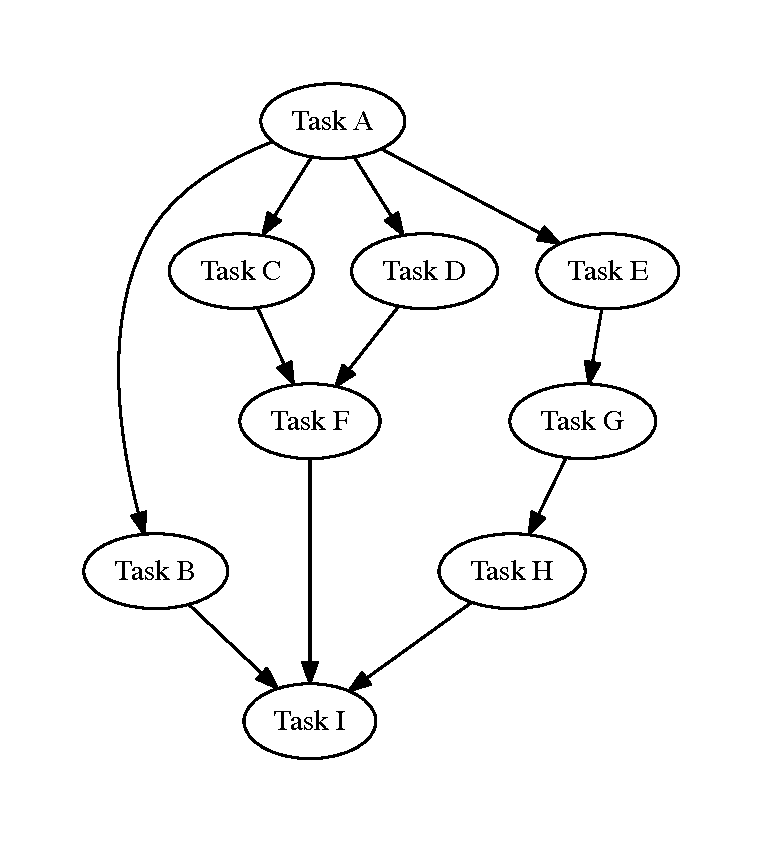
\includegraphics[width=120mm]{figures/task_dag_example.pdf}
  \caption[Example of work-span model task DAG]{An example of a task DAG used in the work-span model. Assuming each task takes
    time 1 to complete, this DAG has a \textit{work} of 9 and a \textit{span} of 5.}
  \label{fig:dag_example}
\end{figure}

In the work-span model, the following bound on the speedup $S$ holds:

\begin{displaymath}
  S \leq \frac{T_1}{T_\infty}
\end{displaymath}

With $n$ workers and running time $T_n$, the following speedup condition can be derived:
\begin{displaymath}
  S = \frac{T_1}{T_n} \approx P \text{ if } \frac{T_1}{T_\infty} \gg P
\end{displaymath}

In essence, this means that linear speedup can be achieved under the condition that the work divided by the span is significantly
larger than the number of workers.

The work-span model implies that increasing the work in an excessive manner when parallelizing may result in a disappointing
outcome. It also implies that the span of the program should be kept as small as possible in order to utilize parallelization as
much as possible.
